\documentclass{article}

% PACKAGES =====================================================
% font settings
\usepackage{titlesec}
\usepackage{lmodern}
\usepackage[T1]{fontenc} % For improved sans-serif font
% Change title format to sans-serif
\titleformat{\title}{\sffamily\LARGE\bfseries}{}{0pt}{}
% Change section format to sans-serif
\titleformat{\section}{\sffamily\Large\bfseries}{}{0pt}{}
% Change subsection format to sans-serif
\titleformat{\subsection}{\sffamily\large\bfseries}{}{0pt}{}
% Change subsubsection format to sans-serif
\titleformat{\subsubsection}{\sffamily\normalsize\bfseries}{}{0pt}{}
% page settings
\usepackage[a4paper,scale=0.8]{geometry}
% language settings
\usepackage[american]{babel}
% captions settings
\usepackage{caption}
\captionsetup{labelfont={small,sf,bf}}
\setlength\belowcaptionskip{5pt}
% graphics settings
\usepackage{graphicx}
% tweaking the footnotes
\usepackage[hang,flushmargin]{footmisc}
% bibliogrpahy
\usepackage[backend = biber, autolang=other, style = nature]{biblatex}
\addbibresource{my_bib.bib}
% graph creation
\usepackage{tikz}
\usepackage{float}
% hyperref
\usepackage{hyperref}
% table settings
\usepackage{multirow}
\usepackage{csvsimple}
% float barrier
\usepackage{placeins}
% list settings
\usepackage{enumitem}
% figure settings
\usepackage{subcaption}

% maths settings
\usepackage{amsmath}
\usepackage{amssymb}

\usepackage{listings}
\usepackage{xcolor}
\lstset{
  basicstyle=\ttfamily,
  keywordstyle=\color{blue},
  commentstyle=\color{green!60!black},
  stringstyle=\color{orange},
  showstringspaces=false,
  numbers=left,
  numberstyle=\tiny\color{gray},
  stepnumber=1,
  numbersep=5pt,
  breaklines=true,
  frame=single,
  tabsize=2,
  captionpos=b
}


% header settings
\usepackage{fancyhdr}
\pagestyle{fancy}
\fancyhf{} % Clear all header and footer fields
\fancyfoot[C]{\thepage} % Add page numbering to the center footer

\renewcommand{\headrulewidth}{0pt} % Remove horizontal line from header
% first page customization
\fancypagestyle{plain}{
\fancyhead[L]{\textit{Lisa PARUIT}- Statistics in R Assessment}
% Left header
  \fancyhead[R]{
%    \raisebox{-0.3\height}{\includegraphics[height=1cm]{Premier_logo.jpg}}
    \raisebox{-0.3\height}{
\includegraphics[height=0.9cm]{Imperial-logo.png}}
  }}

% title settings
\title{\sffamily\LARGE\bfseries Annual and Long-term Variability in Oak Trees Phenology }
\author{\sffamily Statistics in R Assessment\\Lisa PARUIT}
\date{}

% BEGIN DOC ====================================================

\begin{document}
\maketitle

% Changement du titre de l'environnement abstrac
% La créationd 'un second environement abstract est possible en réitérant cette série de lignes

% =======================================================================

\vspace{-1cm}

\section{Introduction}\label{sec:intro}

It is well established that the timing of leaf unfolding in temperate deciduous trees is influenced by environmental cues, particularly chilling and forcing accumulation \cite{Fu_2013}. However, from year to year, we observe a variability in the distribution of leaf unfolding dates (cf. \autoref{fig:forcing_doy_chilling}), as well as differences in the shape of the distribution on an annual basis (cf. \autoref{fig:histogram_doy_year}). In this study, we aim to investigate the mechanism behind this annual and long-term variability, thereby improving our understanding of the temporal distribution of spring phenologic events in oak trees (\textit{Quercus robur}). 

\begin{minipage}[t]{0.45\textwidth}
\begin{figure}[H]
    \centering
    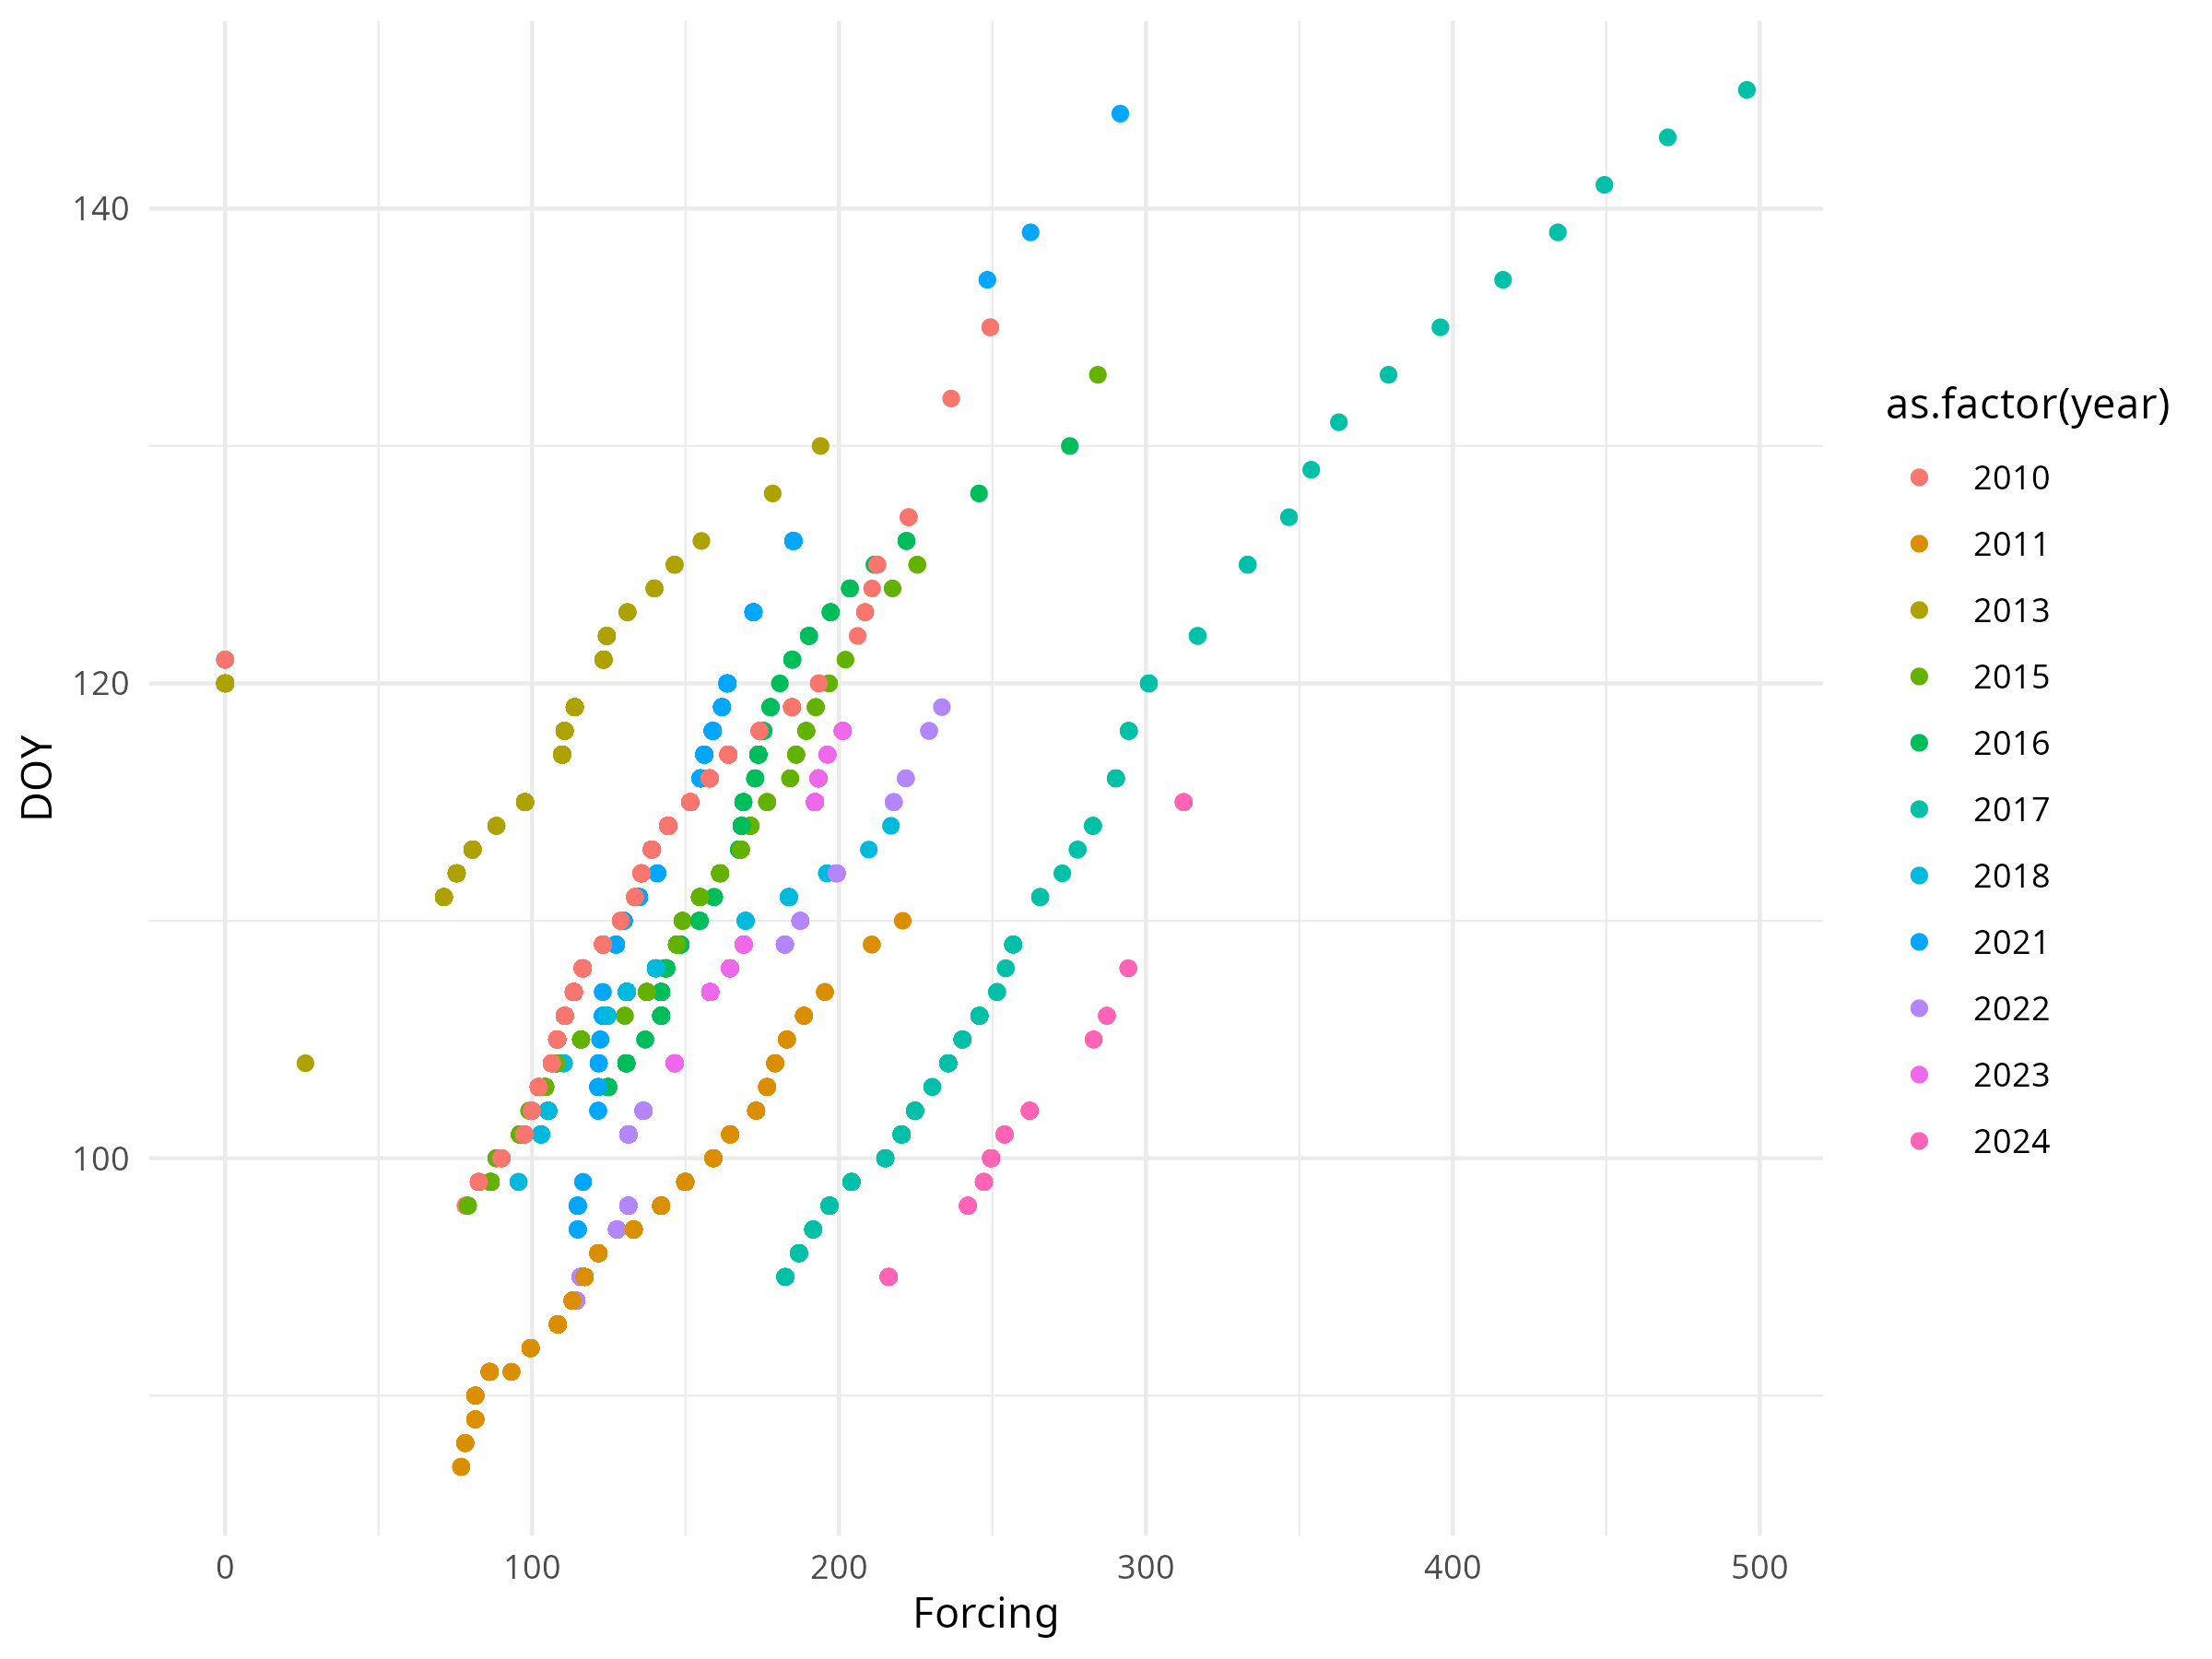
\includegraphics[width=\textwidth]{Forcing_vs_DOY_by_Year.png}
    \caption{Relationship between Forcing and Day of Year (DOY) of bud burst, colored by Chilling levels (ie. years).}
    \label{fig:forcing_doy_chilling}
\end{figure}
\end{minipage}
\hfill
\begin{minipage}[t]{0.45\textwidth}
  \begin{figure}[H]
    \centering
    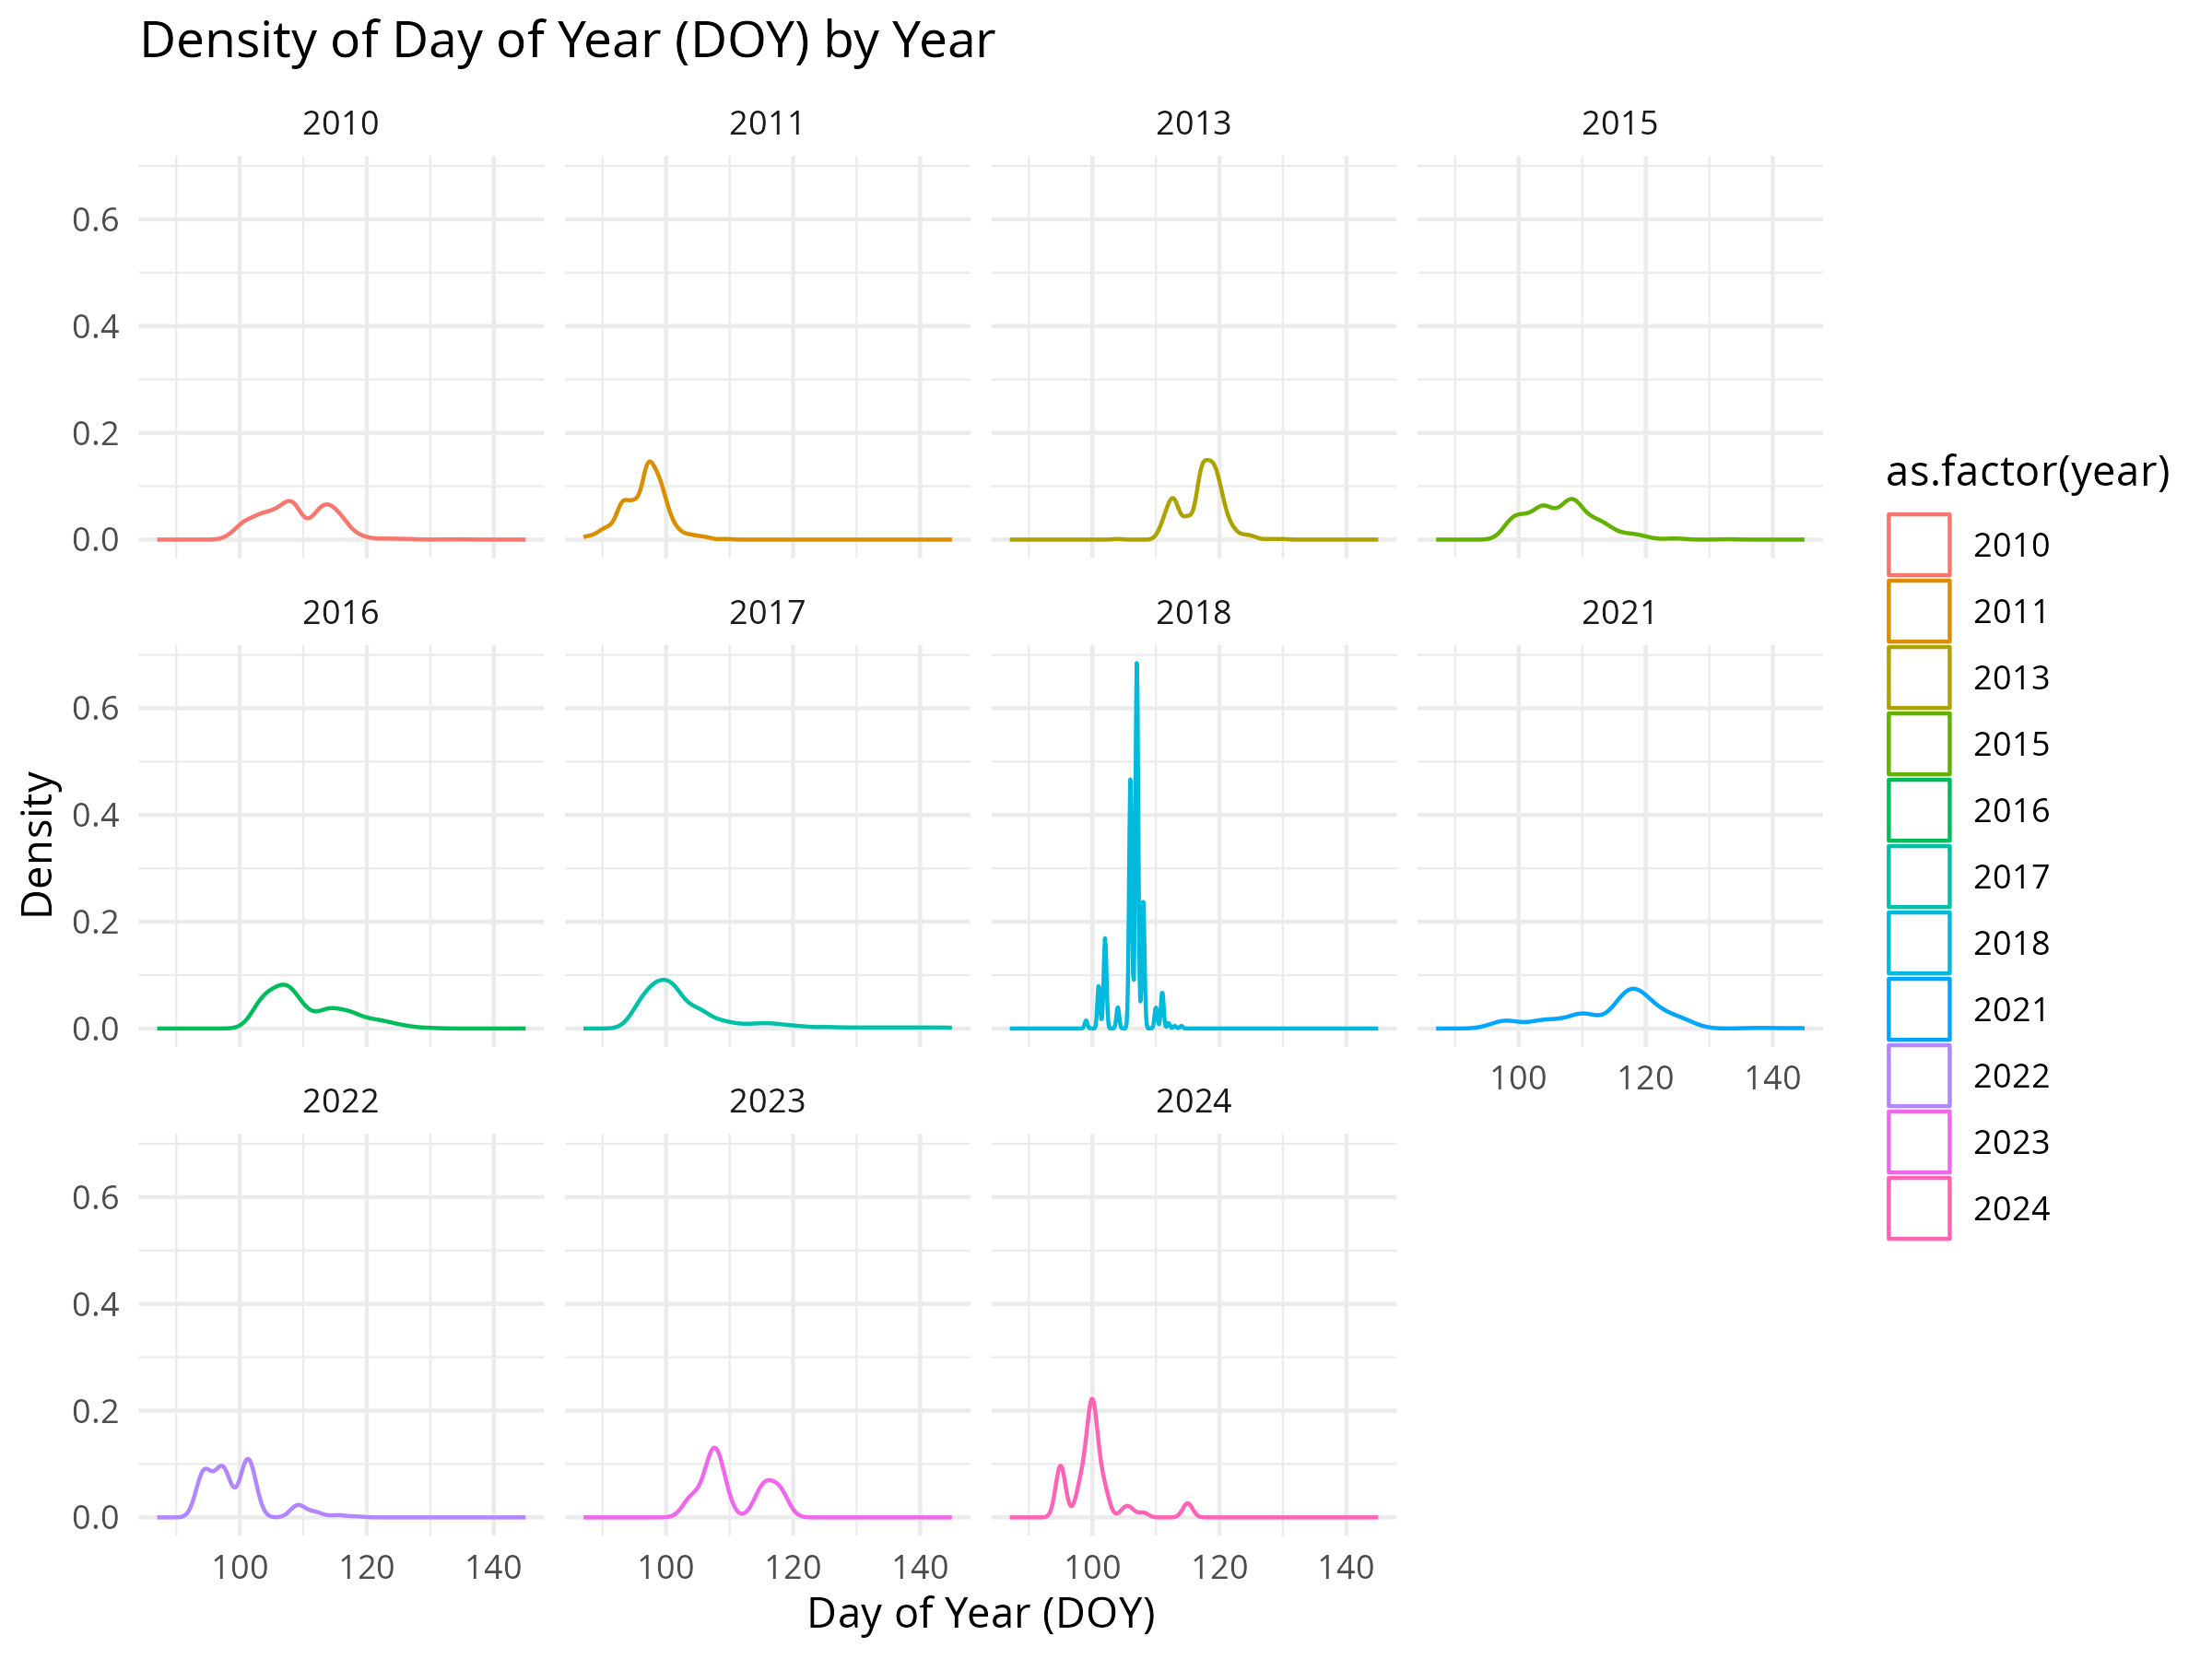
\includegraphics[width=\textwidth]{Density_DOY_by_Year.png}
    \caption{Density of bud burst events, faceted by year. Each panel represents the distribution of the DOY for a specific year.}
    \label{fig:histogram_doy_year}
  \end{figure}
\end{minipage}

\section{Methods}\label{sec:methods}

\paragraph{Parameters}
Forcing and chilling were computed using (Fu et al., 2013)'s formula \cite{Fu_2013}. In addition to forcing and chilling, we considered environmental variables such as rainfall accumulation and location in Silwood Park. Physiological variables include tree girth (as a proxy for age) and tree form.\\
Date of bud burst was obtained from the dataset provided using a standardized method. When unclear ($<1$ or $>1$ notations), we respectively used the next and previous day after or prior observation when this was not a visit day. When not applicable, we used the date of the closest observation. 

\paragraph{Variable selection on fixed effect model}
An LMM incorporating all variables as fixed effects shows some deviation from normality in the residuals distribution. Therefore, we considered a GLM with a Gamma-distributed response variable to better capture the data characteristics (cf.\autoref{lst:mod3_code}). \\
On \autoref{fig:glm_diagram}, one can see that the residuals vs fitted plot shows there is some heterscedasticity, yet expected in Gamma models. The QQ plot shows that this model choice is very satisfactory as the residuals closely follow the theoretical quantiles line. The scale location plot shows a random scatter around zero, indicating homoscedasticity of the residuals. Finally, the residuals vs leverage plot shows some outliers though not changing the overall fit of the model. 


\begin{minipage}[t]{0.45\textwidth}
\begin{table}[H]
\centering
\begin{tabular}{lrrrc}
  \hline
 & LR Chisq & Df & Pr($>$Chisq) \\ 
  \hline
Chilling & 139.9947 & 1.0000 & 0.0000 & ***\\ 
  Forcing & 219.7402 & 1.0000 & 0.0000 & ***\\ 
  Rain & 189.6201 & 1.0000 & 0.0000 & ***\\ 
  girth\_cm & 253.8346 & 1.0000 & 0.0000 & ***\\ 
  TreeForm & 5.6314 & 1.0000 & 0.0176 & *\\ 
  SPlocation & 321.8154 & 33.0000 & 0.0000 & ***\\ 
   \hline
\end{tabular}
\caption{Analysis of Variance (ANOVA) table for the Gamma GLM (mod2).}\label{tab:anova_mod2}
\end{table}

\begin{lstlisting}[language=R,caption={GLM used to select relevant variables in general budburst distribution},label={lst:mod3_code}]
mod2 = glm(DOY ~ Chilling + Forcing + Rain + girth_cm + TreeForm + SPlocation, data = Data, family = Gamma(link = "log"))
\end{lstlisting}


\end{minipage}
\hfill
\begin{minipage}[t]{0.45\textwidth}
\begin{figure}[H]
    \centering
    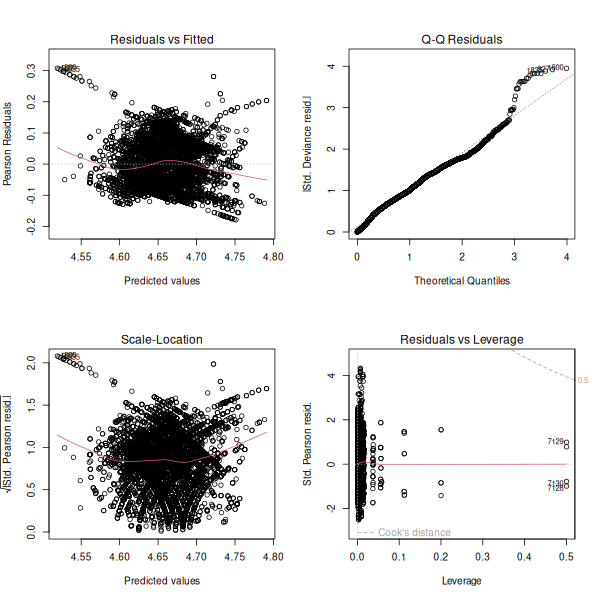
\includegraphics[width=0.9\textwidth]{mod2_diagnostics.png}
    \caption{Diagnostic plots for the Gamma GLM (mod2)}
    \label{fig:glm_diagram}
\end{figure}
\end{minipage}

\noindent \autoref{tab:anova_mod2} shows the results of the ANOVA performed on each level of the model. The tree form variable has the highest p-value (0.0176). We will therefore consider removing it in the next steps. 




\section{Results}\label{sec:results}%%%%%%%%%%%%%%%%%%%%%%%%%%%%%%%%5

\paragraph{Mixed effect model with random intercepts per year}
To account for potential year-to-year variability not captured by the fixed effects, we introduced random intercepts for each year in a mixed-effects model framework (cf. \autoref{lst:mod3_code}).
The anova performed on this model, summarized in \autoref{tab:anova_mod3},shows that the annual distribution of bud burst dates is significantly impacted by the variables Forcing, rain and Location. This suggest that Chilling and girth may be the cause of annual variation.

\begin{table}[ht]
\centering
\begin{tabular}{lrrrc}
  \hline
Term & Chisq & Df & Pr($>$Chisq) & \\ 
  \hline
Chilling & 0.8420 & 1.0000 & 0.3588 & \\ 
  Forcing & 50268.8994 & 1.0000 & 0.0000 & *** \\ 
  Rain & 4291.8768 & 1.0000 & 0.0000 & ***\\ 
  girth\_cm & 3.5864 & 1.0000 & 0.0583 & . \\ 
  SPlocation & 121.1303 & 25.0000 & 0.0000 & *** \\ 
   \hline
\end{tabular}
\caption{Analysis of Variance (ANOVA) table for the mixed-effects model with random intercepts per year (mod3).}\label{tab:anova_mod3}
\end{table}

\noindent The summary of the model coefficients (not presented here) also shows that some locations have a significant effect on the bud burst dates distribution. In particular, Gunnes's hill, Hell hill, Mann's Copse, Merten's Acres, Pound Hill Field and Rookery Slope all have a very significant negative effect on the bud burst dates, indicating that trees in these locations tend to burst their buds earlier in the year compared to the reference location. This could be due to microclimatic conditions or soil characteristics specific to these locations that promote earlier bud burst.

\begin{minipage}[t]{0.4\textwidth}
\begin{figure}[H]
    \centering
    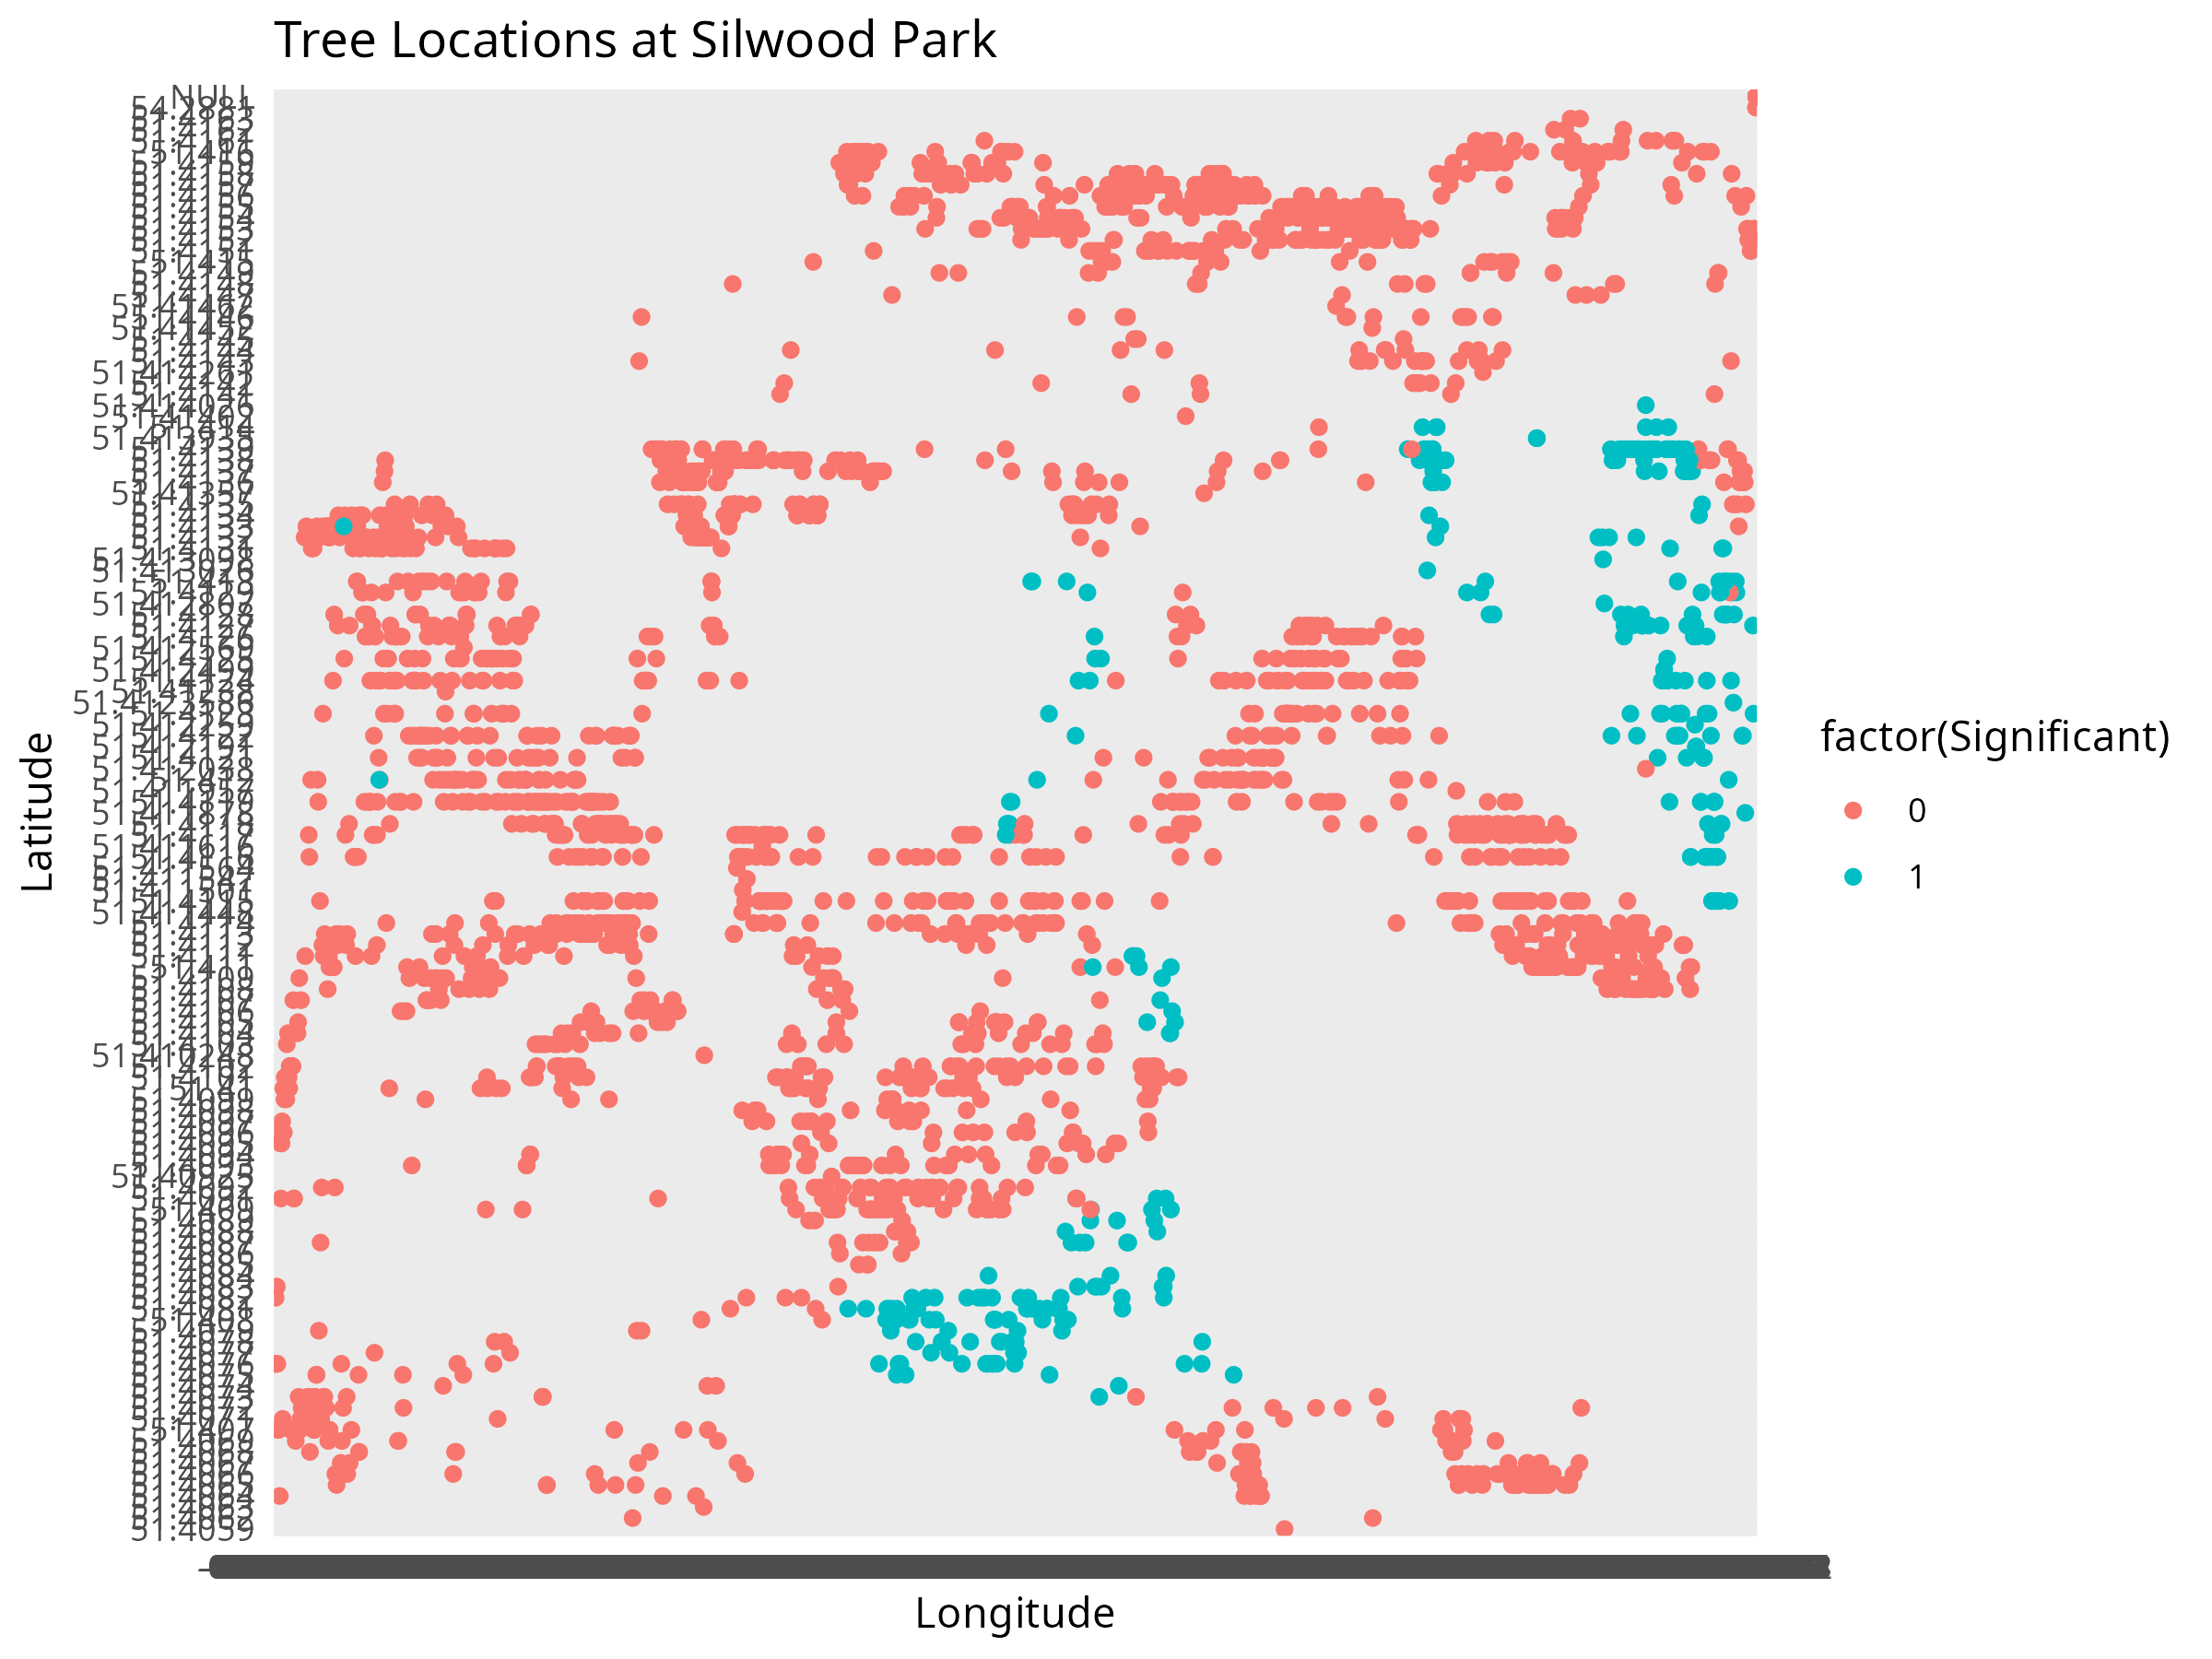
\includegraphics[width=\textwidth]{Tree_Locations.png}
    \caption{Tree Locations at Silwood Park in a longitude/latitude coordinate plane. Locations with significant negative effect on bud burst dates are highlighted.}
    \label{fig:tree_locations}
\end{figure}
\end{minipage}
\hfill
\begin{minipage}[t]{0.55\textwidth}
 On \autoref{fig:tree_locations}, we can see the spatial distribution of the trees in Silwood Park. The locations with significant negative effects on bud burst dates do not seem to be clustered in certain areas, suggesting that there is no large scale pattern in the spatial distribution of these effects. However, the name of these locations (e.g. "hill", "slope", etc.) suggest that they may be associated with specific topographical features that could influence microclimatic conditions and thus bud burst timing.

 \begin{lstlisting}[language=R,caption={GLM of the gamma family with mixed effect, using significant fixed effects on DOY distribution as predictors and random intercepts per year.},label={lst:mod3_code}]
mod3 = glmer(DOY ~ Chilling + Forcing + Rain + girth_cm + SPlocation + (1|year), data = Data, family = Gamma(link = "log"))
 \end{lstlisting}

\end{minipage}

\paragraph{Investigating the effect of chilling and girth size}
To further investigate the influence of chilling and girth size on the inter-year variability of bud burst precocity, we fitted a linear model with interaction for the intercept of the previous model with these two predictors. \\
In \autoref{tab:summary_mod4}, we can see that chilling seems to be the key variable here with a significant negative effect of the intercept of the yearly bud burst dates distribution. Although, the adjusted R-squared of the model is relatively low (0.05146) and the QQ-plot shows that the chosen model fits the data quite poorly.

\begin{minipage}[t]{0.6\textwidth}
\begin{table}[H]
\centering
\begin{tabular}{rrrrrc}
  \hline
 & Estimate & Std. Error & t value & Pr($>$$|$t$|$) \\ 
  \hline
(Intercept) & 0.2480 & 0.0187 & 13.2951 & 0.0000 & ***\\ 
  Chilling & -0.0043 & 0.0003 & -12.6442 & 0.0000 & *** \\ 
  girth & -0.0003 & 0.0001 & -2.3627 & 0.0182 & *\\ 
  Chil:girth & 0.0000 & 0.0000 & 2.2518 & 0.0244 & *\\ 
   \hline
\end{tabular}
\caption{Summary of the linear model investigating the effect of chilling and girth size on bud burst dates.}\label{tab:summary_mod4}
\end{table}

\begin{lstlisting}[language=R,caption={Linear model used to investigate the effect of chilling and girth size on yearly bud burst dates variation.},label={lst:mod4_code}]
mod4 <- lm(int ~ Chilling * girth_cm, data = intercepts_data)
\end{lstlisting}

\end{minipage}
\hfill
\begin{minipage}[t]{0.35\textwidth}
\begin{figure}[H]
    \centering
    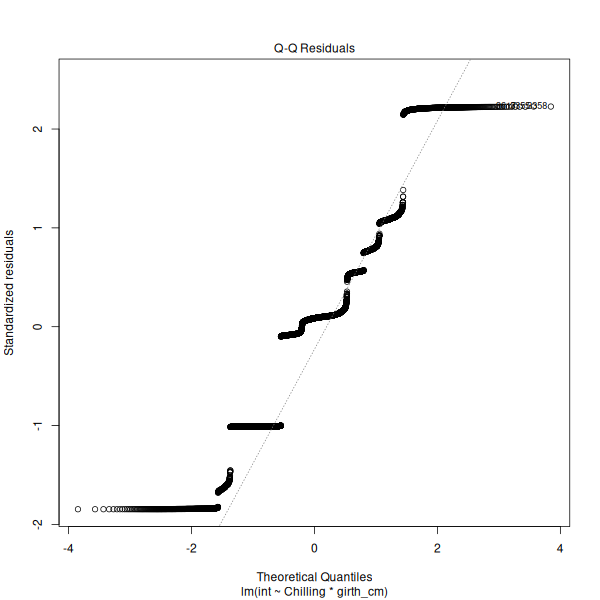
\includegraphics[width=0.9\textwidth]{mod4_diagnostics.png}
    \caption{Q–Q Plot of Residuals for the linear model investigating the effect of chilling and girth size on bud burst dates (mod4).}
    \label{fig:mod4_qq}
\end{figure}
\end{minipage}


\vspace{-0.5cm}
\section{Conclusion}\label{sec:conclusion}
This study aimed to investigate the variables related to annual and long-term variability in bud burst dates of \textit{Quercus robur} in Silwood Park. By employing a mixed-effects modeling approach, we identified that forcing accumulation, rainfall, and micro-climatic condition (potentially exposure) significantly influence the timing of bud burst on an annual basis. However, it appeared that chilling is the main variable contributing to inter-annual variability, although results suggest that other unrecorded factors may also play a role in this phenomenon. Morevover, long-term trends in spring phenological events date is very likely to be influenced by global warming, which impact many variables in a non-linear and complex manner. This deduction is therefore out of the range of this study and would require further investigation using more sophisticated modeling techniques and additional data.

\printbibliography
\end{document}